\documentclass[a4paper, 11pt, oneside, polutonikogreek, latin]{article}
\usepackage[T1]{fontenc}
\usepackage{Alegreya} %% Option 'black' gives heavier bold face 
\renewcommand*\oldstylenums[1]{{\AlegreyaOsF #1}}

% Load encoding definitions (after font package)

\usepackage{textalpha}

\usepackage{listings}
\lstset{basicstyle=\ttfamily}

% Babel package:
\usepackage[latin]{babel}

% With XeTeX$\$LuaTeX, load fontspec after babel to use Unicode
% fonts for Latin script and LGR for Greek:
\ifdefined\luatexversion \usepackage{fontspec}\fi
\ifdefined\XeTeXrevision \usepackage{fontspec}\fi

% "Lipsiakos" italic font `cbleipzig`:
\newcommand*{\lishape}{\fontencoding{LGR}\fontfamily{cmr}%
		       \fontshape{li}\selectfont}
\DeclareTextFontCommand{\textli}{\lishape}

\usepackage[dvipsnames]{xcolor}
\usepackage{eso-pic,graphicx}
\usepackage[top=70mm, bottom=65mm, outer=28mm, inner=28mm]{geometry}
\setlength{\columnsep}{90pt}

\definecolor{customColor}{RGB}{85, 0, 255}

\usepackage{sectsty}
\usepackage[titles]{tocloft}

\usepackage{setspace}
\onehalfspacing

\usepackage{booktabs}
\setlength{\emergencystretch}{15pt}
\usepackage{fancyhdr}
\usepackage{microtype}
\usepackage{sectsty}
\sectionfont{\Huge\bfseries}
\subsectionfont{\LARGE\bfseries}

% change color of text, example replace all \color{Goldenrod} with \color{lightgray}

\makeatletter % change only the display of \thepage, but not \thepage itself:
\patchcmd{\ps@plain}{\thepage}{\bfseries\large\color{customColor}{\thepage}}{}{}
\makeatother

\color{customColor}

\begin{document}
\bfseries
\renewcommand{\contentsname}{
\bfseries{Index}
}
\renewcommand\thefootnote{{\arabic{footnote}}}
\let\oldfootnote\footnote
    \renewcommand{\footnote}[1]{\oldfootnote{\large#1}}
\AddToShipoutPictureBG{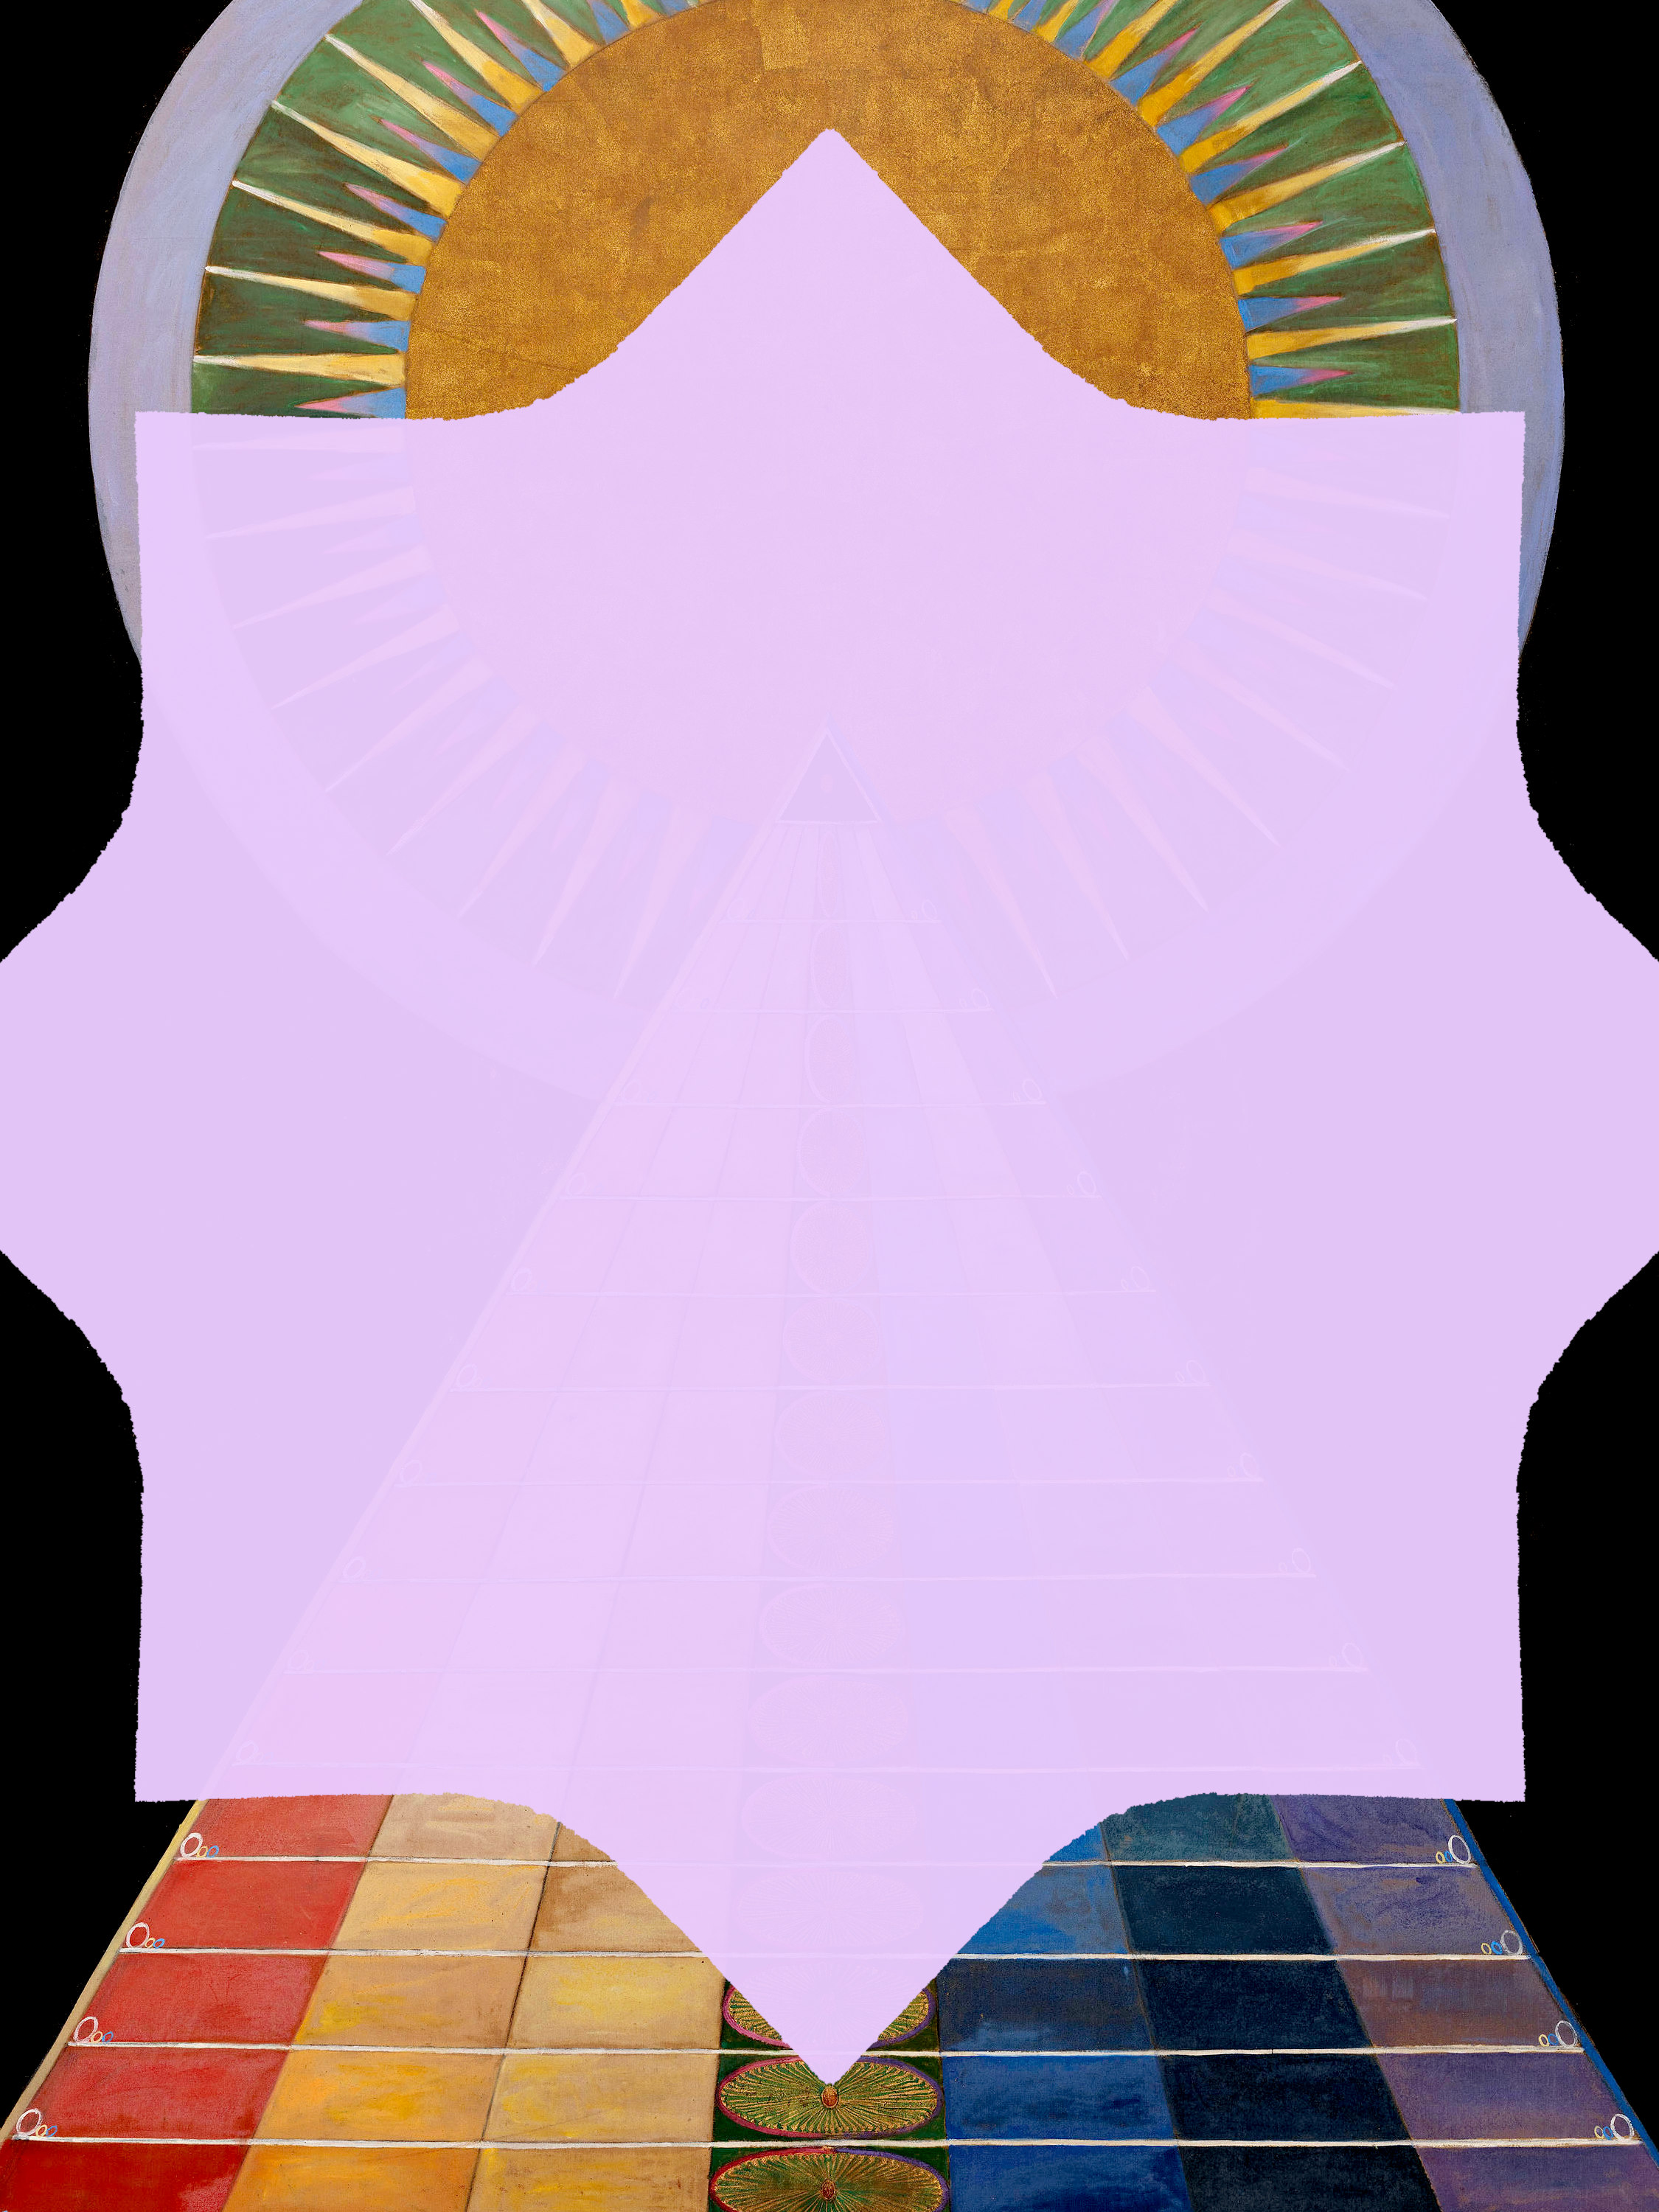
\includegraphics[width=\paperwidth,height=\paperheight]{klint1.jpeg}}
\begin{titlepage} % Suppresses headers and footers on the title page
	\centering % Centre everything on the title page
	%\scshape % Use small caps for all text on the title page

	%------------------------------------------------
	%	Title
	%------------------------------------------------
	
	\rule{\textwidth}{1.6pt}\vspace*{-\baselineskip}\vspace*{2pt} % Thick horizontal rule
	\rule{\textwidth}{0.4pt} % Thin horizontal rule
	
	\vspace{1\baselineskip} % Whitespace above the title
	
	{\scshape\Huge De Pluvia Lapidea.}
	
	\vspace{1\baselineskip} % Whitespace above the title

	\rule{\textwidth}{0.4pt}\vspace*{-\baselineskip}\vspace{3.2pt} % Thin horizontal rule
	\rule{\textwidth}{1.6pt} % Thick horizontal rule
	
	\vspace{1\baselineskip} % Whitespace after the title block
	
	%------------------------------------------------
	%	Subtitle
	%------------------------------------------------
	
	{\scshape \Large Ad Strkow et Ejus Causis Meditatio.} % Subtitle or further description
	
	\vspace*{1\baselineskip} % Whitespace under the subtitle
	
        {\scshape Per Josephum Stepling,\\Soc. Jesu Sacerdotem, Cæsareo-Regium Studii Philosophici Pragensis, et Artium. } % Subtitle or further description
    
	%------------------------------------------------
	%	Editor(s)
	%------------------------------------------------
        \vspace*{\fill}

	\vspace{1\baselineskip}

	{\small\scshape Anni 1753.}
	
	{\small\scshape{}}
	
	\vspace{0.5\baselineskip} % Whitespace after the title block

        \scshape Internet Archive Online Edition  % Publication year
	
	{\scshape\small Attribution-NonCommercial-ShareAlike 4.0 International} % Publisher
\end{titlepage}
\setlength{\parskip}{1mm plus1mm minus1mm}
\clearpage
\tableofcontents
\clearpage
\Large
\pagestyle{fancy}
\fancyhf{}
\cfoot{\bfseries{\thepage}}
\section[Dedicatio.]{\bfseries{Dedicatio.}}
\paragraph{}
Non ars solum inventis, sed et natura insolitis Phænomenis hoc ingenuo, quod vivimus, sæculo Philosophis patrocinari videtur: ut habeant, quo eruditis cogitationibus et mentem occupent, et rerum natur alium scientia publico prosint. E pluribus unum recitabo, quod anno superiore in Bohemia haud longe ab urbe Thabor in vicinia Strkoviensi accidisse etiam per mitteras accepimus, sparsiex improviso per campos lapides videbantur, quos an nubes gravida effuderit? an ventus potentior collectas attulerit? an denique motus insolentior e terræ visceribus ejecerit, incertum fuerat spectantibus.

Præbuit hæc rei novitas occasionem Philosopha in causas rei tam insolitæ solertius indagandi, ventorum vim, atque potentiam expendendi; quid sapienter denique de hoc ominari, quid decerni possit, dissertatione complectendi.

Luæ cum et eruditione plena sit, et rerum naturalium sciendarum cupidis peramœna, TUIS ausus sum honoribus dicare EXCELLENTISSIME Domine, Domine Patrone. Hac et meum TIBI grati animi studium, quod ipsa adeo ætate majus est, testari volui, et simul propensam TUAM, qua literas æque, ac literatos proseuqeris volunatatem orbi commendare.

Luamvis vel me tacente Scholæ, Gymnasia, Universitates, omnisque Eruditorum societas hoc fateatur, qui vel exemplis TUIS, vel eruditis speciminibus, aut certe sermonibus atque disucrsibus eruditis se se adjutos gloriantur.

Inde vero cui mirum sit amplius, quod tanta sapientiæ TUÆ fama regnum universum pervaserit? quod in remotas etiam provincias penetraverit? quod denique in Aula tanti æstimata fuerit, ut non uno, sed compluribus, quibus vix permulti alii pares forent, dignitatibus fueris ornatus. Sed molesta, adverto, hæc TUÆ sunt modestiæ, qui pene magis TUARUM laudum pertæsus es, quam alii laborum. Præteribo igitur avitam generis TUI nobilitatem, præteribo Majorum TUORUM officia, munera, honores, gesta præclare facinora, TE ipsum denique potissima TUI parte id est singularem TUAM in Superos pietatem, in miseros clementiam, in singulos humanitatem pæteribo. Luanquam hæc ipsa decora ita ante omnium oculos versantur, ut nemo unus sit, qui non vitam TIBI incolumem, sibi felicitatem TE fruendi porro, TUIS LUE virtutibus incitari exoptet.

Ego certe, qui spectatis exemplis TUIS ad literarios conatus incitatus Philosophicam arenam subeo, disceptationem meam honori TUO consecro, id simul recipiens, nunquam me commissurum, quo minus meum in TE colendo desiderium, in exoranda, TIBI, diuturna vitæ incolumitate studium elucscat.
\begin{center}
EXCELLENTISSIMI DOMINI
\end{center}
\begin{center}
Minimus et perpetuus Cliens Antonius Hoering.
\end{center}
\clearpage
\section[Ad Lectorem.]{\bfseries{Ad Lectorem.}}
\paragraph{}
Habes benevole lector, quae inter crebra et cumulata mense præprimis Aususto muniorum meorum negotia horulis subsecivis meditatus sum. Nunquam quidem in mentem venit ea luci publicæ committere, cum Eruditiorum seculi nostri lectorm expectationi facturum me omnino satis vix putarem, propterea, quod certiora quædam, eaque ad quaestionem praesentem plene decidendam magis opportuna adhuc defiderentur. Feci attamen, quod id dandum censui amico petenti, et quod opportunum putavi: specimine edito palam facere, iis in consessibus, quos instituente atque imperante Maria Theresia Augusta Patriæ et Musarum Matre celbramus, non remote sive a tempore, sive cognitione et sensu nostro nos perscrutari, sed quæ sint ante pedes, sed quæ ad naturæ revelanda arcana conducant, aut sua se se utilitate sive in scientiis sive vita communi commendent. Itaque lucubratiunculam istam æqui bonique consulito; neque si tibi forte non placeat, aut probetur, continuo displicituram omnibus velim perfuadeas. Vale.
\clearpage
\section[Historia pluviæ lapideæ ad Strkow.]{\bfseries{Historia pluviæ lapideæ ad Strkow.}}
\paragraph{}
Cogitanti mihi, quo ordine præsentis quæstionis solutio pertractanda foret, factu optimum visum est: principio ipsam hujus pluviae lapideae historiam una cum suis circumstantiis, quae quidem ad meam pervenere cognitionem, deinceps ejus causas, si evolvi possent, explicatas dare. Cum enim similium effectuum (sæpe autem similes apparent, si, quæ illos præcedunt, comitantur, atque sequuntur, confiderare omittas) diversæ esse possint causæ et origines ad eam, quæ dato in casu obtinuerit, profecto non alia patescit via, quam per adjuncta et circumstantias, hæcque sola tuta est, atque munita, Ita ergo se res habuit. Tertia erat Julii, cum ecce sub horam octavam vespertinam aere tranquillo, cœloque parum nubilo ter tonitru vehemens, boatus tormenti bellici haud absimile, editur, quod fragor continuus, atque solito diutius perdurans exepit, quo demum finito lapides externa specie subnigri, intus cineritii quidpiam præseferentes, ex aere valido cum impetu et sono (scissum is violente aerem indicabat) præcipitantur. Pastorum unus aliquis quatuor lapides ferri ex alto videns, accurrit, cum inde abesset passibus non amplius triginta, solo levavit unum, et asservavit. Hæc trans piscinam ad Strkow pagum, uno milliari Taborio dissitum, ita, uit recensui, contigerunt.

Porro alius quidam famulus ex pago Plan ad Toparchiam Strkowiensem pertinente hæc memoriæ prodidit: se in pascuis deciduos cœlo lapides spectavisse omnino, a quibus quinquaginta fere passus abfuerit: in duos imprimis, se ie oculos defixisse, quos terræ allisos pulverem, atque aliquem etiam terræ tremorem concitasse viderit, unum ex eis manu a se attrectatum, non parum calentem reperisse. etc. Ita habet relatio ab Illustrissimi de Wratislaw Territorio, seu, ut ajunt Districtui Bechinensi Præfecto Pragam ad Supremum Consilium Regium, \emph{Repræsentationem} vocant, data. Verum quoniam narratio ista plurium haud meminit circumstantiarum, quarum tamen in in causis eruendis necessaria sit cognitio: quæsita concinnavi, quibus modus, ratioque omnis pluviæ hujus in apricum producer etur, ea rogatu meo nostratium quidam ad Virum plurimum Reverendum D. Josephum Klastersky Taborii Decanum misit, qui pro ea, qua est, humanitate, non gravate ad quædam respondit, atque superiora quidem confirmavit, alia vero etiam adjunxit, nempe: coruscavisse paulum ante, quam trinum illud tonitru auditum fuerit: pluviam ordinariam nullam, neque ventum vehementem se observavisse: lapides in agros partim, partim in piscinas effusos esse, diffugientibus vel domum vel sub arbores pastoribus, neque tamen vel hominem vel pecus læsisse: fuisse illis figuram gibbosam et irregularem atque maximum, qui quidem repertus sit, libras tredecim ponderasse. Recensita sic, uti potui, specie facti, seu historia pluviæ lapideæ, causæ ejus nunc indagandæ veniunt. Ostendam fieri non potuisse, ut lapides decidui, in aere illo sublimi generati fuerint, adeoque eos illuc sublatos ad terram delapsos. Dein quibus viribus sublati sint, inquisitum ibo.
\clearpage
\section[Ostenditur lapides non esse generatos in aere sublimi.]{\bfseries{Ostenditur lapides non esse generatos in aere sublimi.}}
\paragraph{}
Nemo, ut puto, dixerit, fieri potuisse, ut igne cœlesti solum contingente lapides Strkowienses ipso in folo conflati fuerint, quod alibi factum novimus. Nam si ita quidem res se habuit, lapides cœlo lapsi non sunt, atqui tamen lapsos esse observatum est et hoc certe sufficit ad opinnionem hanc, si quis eam foveret, labefactandam, atque abolendam accedir, fulmen tantum a nemine tum observatum fuisse, quod pastorem illum, quem lapidem e terra levasse paulo ante narravimus, latere non potuisset, cum non nisi triginta passuum intervallo a loco lapidum, et quod consequens est, etiam fulminis terram ferientis abfuisset. Dein non videtur lapidis materia talis esse, quæ igne potuerit conflari: aliam certe generationis viam et modum in sequentibus indicabimus. Neque tamen propterea lapidum natalem locum nubes censuerim.

Si namque lapides Strkowienses ex alto decidui in aere sublimi generati sunt, necessum est illic fuisse materiam, qua tanquam sibi propria gaudent; ea itaque in sublimi pependit aeri innatans non secus atque nubes, et ab aere sustentata fuit. Quoniam autem liquidum, quale etiam aer, non sustinet nisi corpus, quod liuido sit \emph{specifice} levius, aut certe ejusdem cum liquido gravitatis specificæ; lapidum materiam in aere pendulam ejusdem cum aere gravitatis specificæ fuisse oportet; adeoque halitum et exhalationem pertenuem atque rarissimam. Sic enim aqua, aliaque liquida in aerem a tellure nequaquam attolluntur ante, neque in aere suspensa hærent, quam in vapores tenues et raros fuerint resoluta. Videamus itaque quantum spatium ab unius lapidis materia occupatum fuerit, siquidem sub forma halitus aeri innatavit. Ut spatium istud utcunqne determinare possem, inquisivi, quamnam gravitatem haberet aqua ejusdem cum lapidum aliquo molis seu extensionis. Et cum ad manum non esset lapis integer e numero eorum, qui ad Strkow delapsi sunt, neque lapidis talis notabilis portio: exstaret autem in collectione fossilium Collegii nostri lapis plane simillimus lapidum Strkowiensium, cujus (æquabat autem 4. digitos cubicos Parisinos) gravitatem specificam explorandam sumpsi, deprehendique aquam ejusdem cum lapide voluminis ponderare unciam unam, drachmas 5. grana 16. Lapidis porro pondus erat 5. unciarum, drachmarum 2. granorum 54. unde lapidis gravitas specifica est ad gravitatem specificam aquæ, ut 2574. ad 796. hoc est, ut 26. ad 8. circiter; quare gravitas lapidis ad gravitatem aeris nostri sub eodem volumine est, ut, 22100. ad 8. seu paulo major quam 2700. ad 1.; itaque halitus ille de quo nobis in præsenti sermo est, si in aere pependisset, spatium bis millies septingenties majus, quam quidem sit magnitudo lapidis, seu spatium pedum cubicorum Parisinorum 75. occupavisset.

Cogitemus jam quo modo, quaque virtute tenuis usque adeo aura et halitus per 75. pedes cubicos diffusus in spatium 4. digitorum cubicorum, seu 2700. minus contrahi potuerit; certe expansam illam materiam momento, et in ictu quasi oculi condensatam fuisse, nemo facile dixerit. Duæ itaque solum supersunt viæ, quibus id fieri potuisse concipiatur: vel enim omnes et singulæ particulæ et moleculæ minimæ exhalationis pedetentim ad se invicem accesserunt, atque inter descendendum (exhalatio enim, cumprimum densior, adeoque aere circumfuso specifice gravior evadit, descensum inchoat) hunc accessum continuantes tandem in densam adeo massam, qualem lapides exhibent abierunt: vel pauculæ moleculæ vicinæ densiores redditæ, adeoque defcendere occœptantes perpetuo alias sibi inter descendendum obvias, atque contiguas arctissimo nexu adjunxerunt, donec tandem in eam molem, tamque duram et compactam, quam lapides præseferunt, excreverint. Si prius? qua, quæfo, vi dispersæ halitus illius particulæ omni ex parte centrum versus inter descensum perpetuo adactæ fuerunt? si dicas? frigus partes illas ignis efficacia divulsas et disjectas rursum constrinxisse: ajo, verum quidem esse, corpora quædam expansa et rarefacta frigore constringi, verum hoc solo sine viribus aliis sociis effici nunquam (nisi forte glacies sit soluta) ut is inter partes dissipatas restituatur nexus, quem ignis sustulit violentia. Ecquis unquam exhalationem ex sulphure sub dio succenso ortam vidit vi frigoris in sulphur coagulari? vapor quidem aquæ ex æolipila erumpens, vitro patentis orificii exceptus, in guttas abit, at non solo frigore, sed quod particulæ violente explosæ in alias vitri cavitati adhærentes irruant, eisque contiguæ cohæreant. Viden? ut præter frigus adsunt alia, quæ illam in guttas resolutionem efficiant? \emph{Sed dices}: Halitum nostrum alio fors superveniente afflatu in lapidem converti utique posse, seu, quod idem, mixtione duarum materiarum subtilium coagulum lapidescens effici.

Verum hæc omnia precario sumis, quin potius fingis, neque enim rei hujuscemodi exemplum adduxeris ullum, et si haud negem, ex duorum liquorum halitu, densiorum mixtione, corpus firmum, et glaciale intra exiguum tempus oriri posse, vix tamen lapidem. Sed demus: quod sumere tibi collibitum fuit; an halitus ille tuus superveniens continuo omnibus partibus halitus in lapidem convertendi adplicabitur? an non potius mixtum hoc in lapillos mole exiles, et guttas velut quasdam lapideas concrescet, quam in lapidem voluminis majoris? istud profecto mihi vero videtur simillimum. Reliquum est, ut si lapides in aere generati sunt, altero ex propositis supra modis generati dicantur. Et hujus quidem modi exemplum habemus in rerum natura: reapse enim, stillæ et grando hac via producuntur: vapores namque altiores, frigore aliquantum condensati, et aere specifice graviores redditi descendere incipiunt, atque in alios aliosque subjectos, et in aere adhucdum  pendulos incidunt, quos sibi adjungunt, et in guttulas minimas, quales habet nebula madefaciens, abeunt, sed perpetuo mole crescunt, vapore, guttulisque aucti, quos inter descendendum contingunt (est enim id proprium plurimis fluidis, ut ubi se contigerint, aut proxime ad contactum accesserint, plures eorum moleculæ omnino cohæreant.). Quodsi eo in loco, ubi primæ illæ ac minutulæ guttæ nascuntur, frigus sit acre satis, ac intensum, guttulæ illæ conglaciantur, atque sub descensum obviis frigore etiam constrictis cohærentes nivium floccos efformant. Sin descendentes guttas majores vel nivium floccos parte aliqua calore solutos, in inferiori regione aeris afflet aura asperior, grando oritur, quæ ad insignem sæpe magnitudinem excrescit; si nempe guttæ conglaciatæ, et descendentes magnæ spissorum vaporum copiæ, aut guttis pluviis obviæ factæ, novis perpetuo corticibus glacialibus involvantur. Quod maxime tum accidere debet, cum vento in transversum abripiuntur, adeoque per magnum spatium vaporibus aut pluvia impletum deferuntur: vel cum grando in grandinem vento illiditur. Dixi grandinem insignis molis exposita ratione oriri posse, qualis certe erat, quam memoriæ prodidit P. Noster de Chales, Tomo 4. \emph{Mundi Mathematici}, ac Romæ Anno æræ vulgaris 1470. decidit magnitudine ovorum struthionis. Collectiones Wratislavienses memorant: Cremæ Anno 1720. sub finem Augusti grandinem 6. librarum, et Anno 1719. Tergesti in Istria frusta glacialia instar globorum ignicreporum, vulgo bombas dicunt, cœlo effusa fuisse. \emph{Dices}: Quin igitur etiam lapides, quorum plurimi 6. libras non æquabant, ita ut grandinem illam magnitudine insignem in aere genitos tenemus? verum non est præcipitandum judicium. Qui grandinem accuratius contemplatus fuerit, inveniet structura, qua gaudet, confirmari modum ortus, quem explicatum dedimus, secuti Patrem nostrum de Chales loco cit. 3. Wolffium aliosque naturæ serutatores. Medium enim grandinis locum communiter nucleus mollior, et niveæ texturæ occupat, quem cortex, imo, si grando major sit, plures etiam cortices, obvolvunt; aut certe vestigia concretionis grandinis inter se collisæ adsunt manisesta. Atqui lapides illi ad Strkow deplui, neque nucleos, neque crustas ostentant, neque ullas concretionis notas. Textura eorum lamellata non est, quod fieri debuisset, si lapidi parvo, seu massæ in lapidem jam induratæ circumfusa fuisset nova materies, huicque induratæ denuo nova accessisset, atque ita deinceps; vix enim credibile est massis lapides constituentibus, simul et semel uniformem adeo per totam extensionem inductam fuisse duritiem. Verum quidem est, crusta tenui subnigra et molliore lapides illos involvi, sed quæ minima sit totius extensionis pars. Dein: cur, amabo, halitus illi, qui condensati ac indurati lapides constituunt, non etiam aliquando saltem molles adhuc, et instar guttarum pluvialium delabuntur? aut cur non lapidibus immixti, uti vapores, qui in grandinem concrescunt, sæpe sub forma guttarum tantum, aut nivium, aut grandinis nivibus, guttisque mixtæ, in campos effunduntur? \emph{Repones} forte istud reipsa accidisse, sulphurque non semel pluisse. Et, ut nihil memorem de antiquioribus temporibus, Anno 1705. Upsalæ igni pluit, ut habet Catonius in Disp. de tellure, citatus a Cla. Wallerio in Hydrologia. Anno 1731. in Galliæ quodam loco Lessay guttæ igneæ velut metallum fusum et candens deciderunr, referente historia A. R. S. ad eundem annum. Guttas has non quidem Sulphur vulgare succensum fuisse (de quo videri potest Neümannus in sua Chymia) oleagineam tamen et inflammabilem quandam materiam, sulphurique analogam, haud eo inficias. At lapidum Strkowiensium materia nihil minus est, atque sulphur; est enim saxea sat copioso, et excocto ferro mixta, ut dicetur. Cæterum quod attinet ad pluviam illam, qua facta, ajunt: sulphur non succensum, sed flavum reperiri, seu pulveres sulphureos flavescentes, ea nulla est. Siquidem pulveres illi ad Regnum Vegetabile pertinent, utpote ex floribus abietum, aliarumque arborum excussi, vide Scheüchzerum \emph{Meteoro. Pag. 14.} Denique lapidum nostrorum compositionem ingrediuntur materiæ, quæ etiam ignis vi volatiles non redduntur, seu in halitum tenuem nequaquam expanduntur. Lapides hi silicum majorum formam præseferunt, non angulosi, sed convexa, irregulari tamen figura præditi. Superficies eis est subnigra, fracti non quidem ex granulis, aut arenulis compositi reperiuntur, neque tamen etiam ad polituram apti fsnt, sed asperi et opaci colore ex cinereo in cæruleum vergente, obscuris flavescentibus maculis, atque etiam metallico, eoque subalbido splendore aspersi, crusta quadam pertenui obvolvuntur, quæ quidem a reliquo lapide non est diversa, neque aliter agnoscitur, quam quod reliquo lapide est aliquantum mollior, ungue facile separabilis, ac friabilis, externaque ejus superficies nigricans. Frustum exiguum lapidis, ad distantiam fere digiti cuspidem acus magneticæ uno pede longæ attraxit, allisumque chalybi scintillas elicuit, sed raras: carbonibus impositum nullum sulphuris odorem efflavit. Lapides istos silicibus adnumerabimus secuti Cla. Wallerium in sua Mineralogia, ubi sub specie silicum opacorum intrinsecus inæqualium et molliorum ponit silicem opacum cærulescentem, dicitque hunc et alios solutos reperiri in tumulis arenariis. D. Reaumur in commentariis A. R. S. ad Annum 1721. Characteres silicum istos reputat: Si fractus lapis arenulis, fibris, aut lamellis contextus non appareat, sed æquabilem: et lævis duritiem Crystallo minimum parem, et aliquam perspicuitatem, quamvis principales notas esse velit illum, quem modo retuli texturæ modum, ac duritiem eam, quæ ad proliciendas chalybis ope scintillas sufficiat. Addi debet, quod Wallerius \emph{Libro cit.} fecit, figura minime angulosa lapidis, sed convexa, etsi irregularis, qualis angulis affrictu multo detritis prodit ; hanc figuram silicibus convenire, etiam ipse celeberrimus Reaumurius \emph{loco nominato} meminit, uti etiam in commentariis Academiæ Regiæ scientiarum ad A. 1723. ubi ex professo de hac figura consueta accuratione disserit.

Neque quo minus lapides Strkowienses silicibus adjungamus, obstat, quod ferrum continent, sive jam illud excoctum sit, sive minus, de quo videbimus. Nam nullum est tam frequens metallum, atque ferrum; in plurimis terrarum speciebus, imo et plantis ferrum reperias: porro ferrum lapidum nostrorum excoctum esse vel inde patet, quod magnetem sentiat.  Multa enim cum veri similitudine ostendit Wallerius \emph{laudato libro}: lapidem, vel terram virtutem magneticam non sentire, nisi actu ferrum contineat. Quodsi itaque lapides Strkowienses silicibus accensendi sint (sive jam silices perfectos, sive imperfectos vocites) tenui arena vel potuis limo, argilave constant, cujus partes minimæ succo lapidifico, seu subtilissima supra modum arena ab aqua limum vel argillam penetrante deposita, firmissime coaluerunt, atque præterea ferreis lapidi immixtis particulis ut ostensum est; quis autem unquam vidit in halitum seu exhalationem resolutum limum vel argillam, aut arenam etsi subtilem, una cum vaporibus in altum evectam? ferrum autem in terram metallicam et phlogiston tanquam principia resolvitur, quorum illud fixum est, atque in tenuem auram expandi vix potest. Itaque nemo rationabiliter asseruerit: hisce ex materiis inter se se sublimi in aere concretis, confusisque, lapides Strkovienses natos fuisse. Denique ne quis objiciat lapides ceraunios dictos, qui in nubibus concuti una cum igne cœlesti evibrari putantur, illud solum adjungo, lapides vulgo pro talibus haberi solitos, esse veterum sive domestica, sive bellica instrumenta, de quibus lege sis Jussieu in commentariis A. R. S. ad Annum 1723.
\clearpage
\section[Lapides Strkowienses e tellure in aerem sunt sublati.]{\bfseries{Lapides Strkowienses e tellure in aerem sunt sublati.}}
\paragraph{}
Cum, ut ostensum in anterioribus, lapides ad Strkow in aere geniti non sint, non aliud superest, quam ut dicamus e tellure in aerem sublatos fuisse, atque inde rursum gravitate propria decidisse. Verum enim vero qua vi in sublime acti fuerint, disputandum nunc venit: vel enim vento, aut turbine extraordinario, aut denique terræ quodam vomitu id factum fuisse oportet, neque certe nunc aliud quid quam, quod dicam, menti succurrit.
\clearpage
\section[Lapides non sunt in aera abrepti procella.]{\bfseries{Lapides non sunt in aera abrepti procella.}}
\paragraph{}
Vento procelloso arbores prosterni, tigna tectorum, atque integra etiam tecta abripi tristis persæpe docuit experientia; cur igitur ex cacuminibus montium vehemente vento flante abripi non possent lapides in superfic ie cacuminis jacentes, soluti penitus, ventique impetui expositi, sicque abrepti in proximas dejici valles, ubi lapidibus pluisse putabitur? ita sane vitulum Avicennæ lanamque pluit: Refert Cardanus \emph{Lib. 16. Subti.} vento sublatum sibi pileum fuisse, cum eques montem Apenninum transiret, additque parum abfuisse, ne portenti vice decideret in proximas villas. Transtulit et equum, cui insidebat, venti violentia ad 2. passus, ita ut fere præcipitaretur. Si tum ibi fuisset exercitus, pileique vento acti in villas ad radices montis sitas dejecti fuissent, rustici pileos pluisse jurassent utique, historicique literis consignassent. Idem Cardanus \emph{loc. cit.} Anno 1618. Mantuæ vento vehementissimo inter alia mulierem pannos lavantem abreptam et per aera longissime asportatam fuisse narrat. Hæc ex Schotti nostri \emph{Phsicæ curiosæ Lib. 11.} verbis illius fere retentis attexere placuit. Attamen solers hic naturæ scrutator, uti et Cabæus nostras sentire videntur: pluvias lapideas nequaquam hac ratione et modo oriri, verum lapides in aere generari, de quo, cum multa jam vera fecerim, non est, quod ultra addam. Istud certum: vento lapides, etiam solutos a superficie telluris, abripi difficulius, quam alia corpora, et si lapidibus absolute graviora, si nempe horum superficies ad gravitatem majorem habeat rationem, quam illorum; majore enim existente corporis firmi superficie major aeris copia in corpus istud incurrit, illudque facilius impellit, et una secum asportat. Cæterum lapides Strkowienses vento vehementi nequaquam in aera abreptos, inde ad tellurem rejectos fuisse, manifestum puto. Neque enim, cum lapides pluit, neque ante, quam pluit, procellam desæviisse narratur; quæ, si adfuisset, cum insignem plane eam fuisse oportuisset, in relationibus datis silentio non fuisset præterita. Quid? quod hæc procella domuum tecta discussisset, arbores postravisset, aliasque strages illa in vicinia edidisset, quorum omnium nil quidquam accidisse compertum habemus.
\clearpage
\section[Lapides Strkowienses non sunt in aera sublati turbine.]{\bfseries{Lapides Strkowienses non sunt in aera sublati turbine.}}
\paragraph{}
Duos tantummodo turbines laconice enarrabo, tum, quod nostra memoria contigere, tum, quod a viris peritissimis atqua doctimissimis recenseantur. Prior accidit Anno 1729. agrumque Ferrariensem, qua parte ad Septemtrionem vergit ultra Padum, male accepit. De eo sermonem scitum, doctumque \emph{Heraclitus Manfredius} conscripsit, atque in Academia scientiarum Bononiensi anno postero recitavit, \emph{commentariorum Instituti Bononiensis Tomo secundo parte altera}, his verbis describitur: \emph{Quietissimo dudum cœlo utebantur} (Trecent incolæ) \emph{nisi quod Evrus spirabat interdum sed lenissime}. \emph{Spirare vehementius cœpit pridie idus} (Augusti) \emph{codemque die ventus Africus exortus est concitatissimus. Hic tum cœlum obduci nubibus, ut, cum hora diei esset secunda jam et vicesima, tempestas maxima imminere videretur; fulgurum tamen nihil erat, inter hæc ingens fragor exaudiebatur, non quasi cœlum tonaret, sed ventus ipse Africus horrendum in modum mugiret; veniebat enim sonitus ex ea parte. Nubes cum aliquanto appropinguassent densissimi fumi speciem, et obscurissimi præseferebant surgentis e terra et late cœlum occupantis. His appropinguantibus grandinavit non nihil sine pluvia, cum propius accessissent, quid esset, apparuit; nam, qui illas inspicere ausi fuerant, testabantur immensum se quasi globum vidisse pulveris, folia intus, cannas, tegulas, tigna, lateres gerentem, que omnia pernicissimo vento rapta, cum alia aliis alliderentur, fragorem edebant tantum; ut quamvis et arbores præteriens turbo exstirparet, et ædificia passim everteret, nihil horum tamen exaudiretur. Velocitate ferebatur tanta, ut qui illum adventantem viderant, et oculis, quoad longissime poterant, prosecuti erant, minutorum sex, septemve spatio e conspectu evasisse crederent; iidemque cum Manfredio id affirmarent, ostendebant agros non exstirpatis tantum arboribus casique dejectis, sed herbis ipsis et satis omnibus absumptis, late vastatos}. Alter turbo, quem commemorare constitui, accidit Anno 1749. Romamque multavit, atque de eo disseruit sermone Italo Pater Rogerius Bosscovich Societatis nostræ. Formam is nubis ad terram usque protensæ referebat, nigræ, flammivomæ, et sulphur exhalantis anter quam Romam contingeret, tonuit cœlum, fulminibus exarsit; cum accederet, ventum violentum, sonumque raucum Romani perceperunt; domus, tum, quas attigit, tum vicinæ, non aliter, atque a terræ motu contremuerunt --- partes illarum disruptæ sunt et dejectæ --- arbores erutæ etc. Hæc desumpta sunt ex \emph{actis Erud. 1753. Mens. Mart. pag. 1.} Ex dictis manifestum est, turbines hujusmodi eos omnes edere effectus, quos venti validi, et si non in turbinem acti, pluresque præterea alios: abripere etiam lateres, consequenter et lapides in altum posse sustollere. Cum autem § \emph{præcedente} dixerimus vento recta excurrente (talem enim tum intelleximus) lapidum Strkowiensium in aera sublationem attribuendam non esse.

Cum alia venti prævalidi, et pernicissimi indicia desint; neque turbini eam elevationem adscribendam esse censuerim; etenim recensiti turbinis effectus, tam ii, quos cum vento prævalido et directo communes habet turbo, quam alii vento in spiras contorto proprii et peculiares pluviam illam lapideam minime sunt comitati.
\clearpage
\section[Lapides Strkowienses videntur ructus quodam terrae, et vomitione in auras ejecti, inde rursum decidisse.]{\bfseries{Lapides Strkowienses videntur ructus quodam terrae, et vomitione in auras ejecti, inde rursum decidisse.}}
\paragraph{}
Relatio de Insula in Archipelago Anno 1707. orta, quam D. Gregorius Condilli in Paro ejusdem Archipelagi insula natus misit ad \emph{Cla. Vallisnierium}, præter alia multa meminit vomitionis lapidum ex fissuris novæ insulæ, quam præcesserunt boatus et rugitus illis tormentorum similes; lapides autem ad infignem altitudinem sublati in distantia trium etiam milliarium ad terram reciderunt. Ex Diario Regiæ Suecicæ scientiarum Academiæ ad Annum 1748. certiores reddimur, anno 1694. ipsis Calendis Januariis sub ortum solis cœlo sereno trinum velut tonitru auditum fuisse in Wærmelandsal, atque tum terræ vomitionem contigisse, qua fossa quadrangularis effecta sit 12 imo decem et sex ulnis profunda, longa vero ex uno latere ulnis 138. Terra ejecta in locum 300. ulnis dissitum recidit. Villa duobus lapidis jactibus dissita ructum hunc nequaquam sensit, atque meridie primum a vicinis de eo, quod accidit, nuntium accepit. Casparus Paragullo in \emph{his. naturali} montis Vesuvii narrat Anno 1631. Vesuvium lapides ingentis molis ad insigne intervallum projecisse, atque unum eorum in Marchionis di Lauro 12. milliaribus Italicis, dissitum injecisse. Quid si igitur et nostri lapides Strkowienses violenta terræ vomitione in auras propulsi fuerunt? non enim in aere orti sunt, non vento procelloso, non turbine eo delati, ut ostendimus, neque superesse modus videtur alius, quo eos aer, qui reddidit, acceperit.

Lapidum pluviam, quod ex omnibus relationibus constat, boatus aliquot præcesserunt; hi nempe e terræ sinu erumpentis repagulaque removentis, erructantisque explosiones fuerunt; quodsi hos spiritus succensos fuisse dicamus, crustulæ nigræ lapides investientis, atque caloris , quo præditi erant, cum deciderunt, ratio non incongrue reddirur; quanquam calor ille etiam abscisso vehementi impetu aere, atque adeo ab frictione, quam lapides passi fuerunt, repeti possit. Certe inflammabilis in aere materiæ succensiones seu fulgetra tanta non præcesserunt, ut iis et boatus illi terrifici, et lapidum calor verosimiliter attribuatur. Verum oggeret unus aliquis, \emph{primo quidem} : dictum fuit ideo lapides neque procella, neque turbine in auras sublatos, quod nullum procellæ et turbinis indicium observatum est, non arbores avulsæ, non domus eversæ, aut tectis spoliatæ; atqui, inquiet, nec terræ motus, ullus nec fissura telluris, et hiatus ullibi, aut flamma et spiritus errumpens est observatus? 2do an cuniculo terrestri, quo soluto lapides in auras exacti sunt, illi tantum lapides ad Strkow inventi incubuere, an non arena (nam in arenariis fere tumulis aut stratis silices reperiuntur) an non alia genera lapidum vel terrarum, quæ itaque etiam in auras evecta, una cum illis lapidibus in agrum Strkowiensem effusa fuissent, quod tamen factum non accepimus. 3tio si lapides terræ ructantis impetu in sublime delati sunt, quid opus erat tempestate, nubibus et fulgetris, quæ tamen lapsum lapidum præcesserunt? Ad hæc quæ objiciuntur sequentia reponenda duxi; et \emph{ad primum} quidem, fateor, necdum me certiorem factum fuisse de fissura aliqua telluris, nec forte ulla huc usque detecta fuit; at neque in talem ex professo inquisitum est: et quid mirum, si fissura non sat ampla, in profundo quodam nemoris recessu, aut deviis montium operta lateat ruricolas, quos late per silvas pagosque editæ procellarum vel turbinum strages latere haud possunt. Quidsi hiatus terræ, ubi spiritus conclusi eruperunt, lateribus coeuntibus hiatus esse desiit? Ad \emph{secundum} ajo, videri vero simile, arenam etiam, terram, aliosque insuper lapides una cum illis cinericeis ejectos fuisse; verum quod ad arenam, terrasque attinet, cum hæ materiæ lapidibus nostris leviores sint, et solutæ, ad minus intervallum propulsæ, reciderunt. Sic sane globus plumbeus e bombarda longius propellitur, atque charta vel alia quævis levior materies, qua ad continendos pulveres pyreos bombarda oneratur. Quod ad lapides attinet alterius speciei, vel ii nostris leviores erant, et tum, ut dixi, ad tantum intervallum propelli non poterant: vel reapse etiam una cum illis cinericeis depluerunt, verum, quod nihil peculiare (quale in illis cinericeis est crusta subnigra) præseferrent, putatum est eos non primo delapsos esse, sed alias quoque illic jacuisse. Ad \emph{tertium} dico fieri potuisse, ut nulla fuerit fulgurum cum lapidum pluvia connexio, sed illa, et hæc ex diversis causis, suis quæque orta fortuito casu se se invicem consecuta esse: aut certe copiosior vomitionem antecedens halitum e terræ visceribus eruptio nubibus, fulguribusque materiam subministravit. De reliquo quid causæ fuerit, quod lapides non quaquaversus circa cuniculum illum terrestrem in orbem projecti sint, verum in solum agrum Strkowiensem, dictu difficile non est; id enim obliquæ spirituum explosioni et memoratum agrum versus directæ attribuendum esse nemo non judicabit. Neque plura addo: solum profi teor, ita meæ me adhærere sententiæ, ut meliora edoctus (et hercle edoceri cupio) et de circumstantiis, quæ forsan aliud sentiendum esse suadeant, certior redditus, eam continuo mutare paratus sim. Optandum enim vero vehementer, quo omnis illa Strkowiensis vicinia ab rerum peritis perlustrata fuisset, aut perlustraretur diligentius, ut tandem aliquando, tum de pluvia lapidea anni lapsi, tum de aliis etiam, quæ nostra memoria in Bohemia acciderunt, explorati aliquid afferri in medium possit. Ter non ita multum disjunctis temporibus lapides pluisse narratur; anno videlicet 1723. Junii 22da secundum Libeschicium anno 1743. ac denique proxi me superiore. Istud mirandum: lapis, quem a prima pluvia ex hic recensitis asservamus, illis Strkowiensibus per omnia similis est. Operæ pretium foret, inquirere sedulo, utrum alicubi lapides hujusmodi in campo soluti, aut tumulis arenariis jaceant, aut intra telluris, agrique Bohemici viscera concludantur, sed manum de tabula.
\clearpage
\end{document}
